\documentclass[a4paper,10pt]{report}
\usepackage{Cours}
\usepackage{delarray}
\usepackage{fancybox}
\newcommand{\Sum}[2]{\ensuremath{\textstyle{\sum\limits_{#1}^{#2}}}}
\newcommand{\Int}[2]{\ensuremath{\mathchoice%
	{{\displaystyle\int_{#1}^{#2}}}
	{{\displaystyle\int_{#1}^{#2}}}
	{\int_{#1}^{#2}}
	{\int_{#1}^{#2}}
	}}


\begin{document}
% \everymath{\displaystyle}

\maketitle{Chapitre 4}{Applications linéaires}

Dans tout le chapitre, $n$, $k$ et $p$ seront des entiers naturels non nuls et $\mathbb{K}$ désignera $\mathbb{R}$ ou $\mathbb{C}$.

 \section{Généralités}
 
 \begin{Definition}{} Soient $E$, $F$ deux $\mathbb{K}$-espaces vectoriels et $f : E \rightarrow F$ une application. On dit que $f$ est \emph{linéaire} si l'une des trois conditions suivantes (équivalentes) est vérifiée :

\begin{enumerate}
\item $\forall (x,y) \in E^2$, $\forall \lambda \in \mathbb{K}$, \phantom{$f(x+y) = f(x)+f(y)$ et $f(\lambda x) = \lambda f(x)$.}
\item $\forall (x,y) \in E^2$, $\forall (\lambda,\mu) \in \mathbb{K}^2$, \phantom{$f(\lambda x + \mu y) = \lambda f(x) + \mu f(y)$. }
\item $\forall (x,y) \in E^2$, $\forall \lambda \in \mathbb{K}$, \phantom{$f(\lambda x + y) = \lambda f(x) +  f(y)$. }
\end{enumerate}
On note $\mathcal{L}(E,F)$ l'ensemble des applications linéaires de $E$ dans $F$ et plus simplement $\mathcal{L}(E)$ dans le cas où $E=F$.
\end{Definition}

\begin{Definition}{} Soient $E$, $F$ deux $\mathbb{K}$-espaces vectoriels et $f : E \rightarrow F$ une application linéaire. On dit que :

\begin{itemize}
\item $f$ est un \emph{endomorphisme} si \phantom{$E=F$.}
\item $f$ est un \emph{isomorphisme} si $f$ est bijective. Dans ce cas, on dit que $E$ et $F$ sont \emph{isomorphes}.
\item $f$ est un \emph{automorphisme} si $f$ est un endomorphisme bijectif. On note $\textrm{GL}(E)$ l'ensemble des automorphismes de $E$ : c'est le \emph{groupe linéaire} de $E$.
\item $f$ est une \emph{forme linéaire} si \phantom{$F = \mathbb{K}$.}
\end{itemize}
\end{Definition}

\begin{Exemple} Soit $D : \mathcal{C}^1(\mathbb{R}, \mathbb{R}) \rightarrow \mathcal{C}^0(\mathbb{R}, \mathbb{R})$ définie par $D(f)=f'$. Montrons que $D$ est une application linéaire. Est-ce un isomorphisme ?

%\begin{itemize}
%\item Montrons la linéarité : soit $(f,g) \in \mathcal{C}^1(\mathbb{R}, \mathbb{R})^2$ et $\lambda \in \mathbb{R}$. On a :
%$$ D(\lambda f + g) = (\lambda f+g)' = \lambda f' + g' = \lambda D(f)+D(g)$$
%Ainsi $D$ est une application linéaire.
%\item $D$ n'est pas injective : toutes les fonctions constantes ont la même image : la fonction nulle.
%\item $D$ est par contre surjective : si $g \in \mathcal{C}^0(\mathbb{R}, \mathbb{R})$, $g$ admet une primitive sur $\mathbb{R}$ que l'on note $G$. Alors $G$ est dérivable sur $\mathbb{R}$ de dérivée $g$ continue sur $\mathbb{R}$ et ainsi $G$ est de classe $\mathcal{C}^1$ sur $\mathbb{R}$ et l'on a $D(G)=G'=g$. Ainsi, $D$ est bien surjective.
%\end{itemize}

\vspace{5cm}
\end{Exemple}

\begin{Proposition}{}
Soient $E$, $F$ et $G$ trois $\mathbb{K}$-espaces vectoriels, $f \in \mathcal{L}(E,F)$, $g \in \mathcal{L}(F,G)$. Alors :

\begin{itemize}
\item $f(0_E)=0_F$.
\item $\forall (\lambda_1, \lambda_2, \ldots, \lambda_n) \in \mathbb{K}^n$, $\forall (x_1,x_2, \ldots, x_n) \in E^n$,
$$ f( \lambda_1x_1+ \lambda_2 x_2 + \ldots + \lambda_n x_n) = \lambda_1 f(x_1) + \lambda_2 f(x_2) + \ldots + \lambda_n f(x_n) $$
\item $g \circ f \in \mathcal{L}(E,G)$.
\end{itemize}
\end{Proposition}

\begin{Remarque}{} $\textrm{GL}(E)$ est un sous-groupe de l'ensemble des permutations de $E$ muni de la composition.
\end{Remarque}

\begin{ApplicationDirecte} Soient $f$ et $g$ les applications de $\mathbb{R}^3$ dans $\mathbb{R}^2$ définies pour tout $(x,y,z) \in \mathbb{R}^3$ par $f((x,y,z))=(x+z,y-z)$ et $g((x,y,z))= (x+y+1,2z)$. Ces applications sont-elles linéaires ?
\end{ApplicationDirecte} 

\begin{ApplicationDirecte} Soit $h$ l'application qui à $P \in \mathbb{R}_n[X]$ associe $2P-3XP'$. Montrer que $h$ définit un endomorphisme de $\mathbb{R}_n[X]$.
\end{ApplicationDirecte}

\section{Noyau et image d'une application linéaire}

\begin{Theoreme}{} Soient $E$, $F$ deux $\mathbb{K}$-espaces vectoriels et $f \in \mathcal{L}(E,F)$.

\begin{itemize}
\item Si $U$ est un sous-espace vectoriel de $E$ alors $f(U)$ est un sous-espace vectoriel de $F$.
\item Si $V$ est un sous-espace vectoriel de $F$ alors $f^{-1}(V)$ est un sous-espace vectoriel de $E$.
\end{itemize}
\end{Theoreme}

\begin{Demonstration}{}
%
%$\rhd$ Soit $U$ un sous-espace vectoriel de $E$. Rappelons que :
%$$ f(U) = \lbrace f(x) \, \vert \, x \in U \rbrace = \lbrace y \in F \, \vert \, \exists x \in U, \, y=f(x) \rbrace$$
%
%\begin{itemize}
%\item $f(U) \subset F$.
%\item L'application $f$ est linéaire donc $0_F = f(0_E)$ et $0_E \in U$ (car $U$ est un sous-espace vectoriel de $E$) donc $0_F \in f(U)$.
%\item Soient $(z,z') \in f(U)^2$ et $\lambda \in \mathbb{K}$. Par définition, il existe $x_1$ et $x_2$ des vecteurs de $U$ tels que $z=f(x_1)$ et $z'=f(x_2)$. On a donc $\lambda z + z' = \lambda f(x_1)+f(x_2) = f( \lambda x_1+x_2)$ par linéarité de $f$. Or $U$ est un sous-espace vectoriel de $E$ donc $\lambda x_1+x_2 \in U$ et donc $\lambda z + z' \in f(U)$.
%\end{itemize}
%Ainsi, $f(U)$ est sous-espace vectoriel de $F$.
%
%\medskip
%
%$\rhd$ Soit $V$ un sous-espace vectoriel de $F$. Rappelons que :
%$$ f^{-1}(V) = \lbrace x \in E \, \vert \, f(x) \in V \rbrace$$
%
%\begin{itemize}
%\item $f^{-1}(V) \subset E$.
%\item L'application $f$ est linéaire donc $ f(0_E)=0_F$ et $0_F \in V$ (car $V$ est un sous-espace vectoriel de $V$) donc $0_E \in f^{-1}(V)$.
%\item Soient $(x,x') \in f^{-1}(V)^2$ et $\lambda \in \mathbb{K}$. Par définition, $f(x)$ et $f(x')$ appartiennent au sous-espace vectoriel $V$ et donc $\lambda f(x)+f(x')$ aussi. Par linéarité de $f$, on a donc $f(\lambda x +x') \in V$ et ainsi $\lambda x+x' \in f^{-1}(V)$.
%\end{itemize}
%Ainsi, $f^{-1}(V)$ est sous-espace vectoriel de $E$.

\vspace{12cm}
 \end{Demonstration}
 
 \begin{att} La notation $f^{-1}(V)$ ne signifie pas que $f$ est bijective.
 \end{att}
 
 \begin{TheoremeDefinition}{} Soient $E$ et $F$ deux $\mathbb{K}$-espaces vectoriels et $f \in \mathcal{L}(E,F)$.
\begin{itemize}
 \item On appelle \emph{image} de $f$, et on note $\textrm{Im}(f)$, l'ensemble $f(E)$. C'est un sous-espace vectoriel de $F$.
 \item On appelle \emph{noyau} de $f$, et on note $\textrm{Ker}(f)$, l'ensemble $f^{-1}(\lbrace 0_F \rbrace)$. C'est un sous-espace vectoriel de $E$.
 \end{itemize}
 \end{TheoremeDefinition}
 
 Autrement dit,
$$ \textrm{Im}(f)= \phantom{\lbrace f(x) \, \vert \, x \in E \rbrace = \lbrace y \in F \, \vert \, \exists x \in E, \, y=f(x) \rbrace}$$
et
$$ \textrm{Ker}(f) = \phantom{ bla bl a\lbrace x \in E \, \vert \,  f(x)= 0_F \rbrace}$$

\medskip

 \begin{Remarques}{}
\begin{itemize} 
 \item Déterminer l'image de $f$ revient à déterminer les vecteurs $y$ de $F$ admettant un antécédent par $f$.
 \item Déterminer le noyau de $f$ revient à déterminer les vecteurs $x$ de $E$ tels que $f(x)= 0_F$.
 \end{itemize}
\end{Remarques}{}
 
 \newpage
 
 \begin{Exemple} Soit $f : \mathbb{R}^2 \rightarrow \mathbb{R}^2$ l'application linéaire définie par $f((x,y))=(x-y,y-x)$. Déterminons le noyau et l'image de $f$.
 
% \medskip
% 
%\begin{itemize}
%\item Soit $(x,y) \in \mathbb{R}^2$. On a $f((x,y))=(0,0)$ si et seulement si $x=y$ et ainsi $\textrm{ker}(f) = \textrm{Vect}((1,1)) \cdot$
%\item On remarque qu'un élément de l'image est nécessairement de la forme $(X,-X)$ où $X \in \mathbb{R}$ et réciproquement, si on se donne un vecteur $(X,-X)$ avec $X \in \mathbb{R}$, on a $f((X,0))=(X,-X)$. Ainsi :
%$$ \textrm{Im}(f) = \lbrace (X,X) \, \vert \, X \in \mathbb{R} \rbrace =  \textrm{Vect}((1,1))$$
%\end{itemize}

\vspace{7cm}
\end{Exemple}

\begin{ApplicationDirecte} Déterminer le noyau de $f$ et $h$ (applications directes du cours $1$ et $2$).
\end{ApplicationDirecte}

\textbf{Application : Équations différentielles.}

Soient $I$ un intervalle de $\mathbb{R}$ (contenant au moins deux points) et $a : I \rightarrow \mathbb{R}$ continue. On définit une application linéaire $D : \mathcal{C}^1(\mathbb{R}, \mathbb{R}) \rightarrow \mathcal{F}(\mathbb{R}, \mathbb{R})$ par $D(y)=y'-ay$. Le noyau de cette application linéaire est l'ensemble des solutions de l'équation différentielle linéaire et homogène d'ordre $1$, $y'-ay=0$.

\medskip 

En notant $A$ une primitive de $a$ sur $I$ (qui existe car $a$ est continue sur $I$), on a pour toute fonction $y$ de $\mathcal{C}^1(\mathbb{R}, \mathbb{R})$ : 

\begin{align*}
\forall t \in I, \, y'(t)-a(t)y(t) =0& \Longleftrightarrow  \forall t \in I, \, \exp(-A(t))y'(t)- a(t)\exp(-A(t))y(t) = 0  \qquad (\exp >0)\\
 & \Longleftrightarrow  \forall t \in I, \, \exp(-A(t))y'(t)- A'(t)\exp(-A(t))y(t) = 0 \\
 & \Longleftrightarrow  \forall t \in I, \, (y \times \exp \circ (-A))'(t) = 0 \\
 & \Longleftrightarrow  \exists C \in \mathbb{R}, \,  \forall t \in I, \, y(t)  \exp (-A(t)) = C \qquad \hbox{(I est un intervalle)}\\
 & \Longleftrightarrow  \exists C \in \mathbb{R}, \,  \forall t \in I, \, y(t) = C \exp (A(t)) \\
\end{align*}
Ainsi $\textrm{Ker}(D) = \textrm{Vect}(\exp \circ A)$.

\begin{Proposition}{} Soient $E$, $F$ deux $\mathbb{K}$-espaces vectoriels et $f \in \mathcal{L}(E,F)$. L'application $f$ est injective si et seulement si $\textrm{Ker}(f) = \lbrace 0_E \rbrace$.
\end{Proposition}

\begin{Demonstration}{} On procède par double implications.
%
%$\rhd$ Supposons que $f$ est injective.
%
%\begin{itemize}
%\item Par linéarité de $f$ on a $f(0_E)=0_F$ donc $\lbrace 0_E \rbrace  \subset \textrm{Ker}(f)$.
%\item Soit $x \in \textrm{Ker}(f)$. Par définition $f(x)=0_F$ et sachant que $f$ est linéaire, on a aussi $f(0_E)=0_F$ et par injectivité de $f$ on a alors $x = 0_E$. Ainsi $\textrm{Ker}(f) \subset \lbrace 0_E \rbrace$.
%\end{itemize}
%Ainsi on a bien $\textrm{Ker}(f) = \lbrace 0_E \rbrace$.
%
%\medskip
%
%$\rhd$ Supposons que $\textrm{Ker}(f) = \lbrace 0_E \rbrace \cdot$ Soit $(x,x') \in E^2$ tel que $f(x) = f(x')$. Par linéarité de $f$, on a alors $f(x-x')= 0_F$ donc $x-x' \in \textrm{Ker}(f) = \lbrace 0_E \rbrace$ donc $x=x'$. Ainsi $f$ est injective.

\vspace{6cm}
\end{Demonstration}

\section{Applications linéaires et familles de vecteurs}

\begin{Proposition}{} Soient $E$, $F$ deux $\mathbb{K}$-espaces vectoriels et $(e_1, e_2, \ldots, e_n)$ une base de $E$. Fixons une famille $(f_1, f_2, \ldots, f_n)$ de vecteurs de $F$. 

Il existe une unique application linéaire $f \in \mathcal{L}(E,F)$ tel que pour tout $i \in \Interv{1}{n}$, $f(e_i)=f_i$.

Autrement dit, une application linéaire est déterminée par l'image des vecteurs d'une base de $E$.
\end{Proposition}

%\begin{Demonstration}{} On raisonne par analyse-synthèse.
%%
%
%\vspace{7cm}
%%$\rhd$ \emph{Analyse} : soit $f \in \mathcal{L}(E,F)$ tel que pour tout $i \in \Interv{1}{n}$, $f(e_i)=f_i$. Tout vecteur $x \in E$ s'écrit sous la forme :
%%$$ x = \sum_{k=1}^n x_k e_k$$
%%ou $(x_1,x_2, \ldots, x_n)$ sont les coordonnées de $x$ dans la base $(e_1, e_2, \ldots,e_n)$. Par linéarité de $f$, on a :
%%$$ f(x) = \sum_{k=1}^n x_k f(e_k) = \sum_{k=1}^n x_k f_k$$
%%
%%\medskip
%%
%%$\rhd$ \emph{Synthèse} : Pour tout $x \in E$, de coordonnées $(x_1,x_2, \ldots, x_n)$ dans la base $(e_1, e_2, \ldots,e_n)$, on pose :
%%$$ f(x) =  \sum_{k=1}^n x_k f_k$$
%%On montre facilement que $f$ est une application linéaire de $E$ dans $F$ et que pour tout $i \in \Interv{1}{n}$, $f(e_i)=f_i$. L'unicité d'une telle application est prouvée dans l'analyse.
%\end{Demonstration}

\begin{Exemple} Soit $(e_1, e_2, e_3)$ la base canonique de $\mathbb{R}^3$. Donnons l'expression de l'unique endomorphisme $\varphi$ de $\mathbb{R}^3$ vérifiant $\varphi(e_1)= \varphi(e_2)= e_1+e_2$ et $\varphi(e_3)=e_1$.

\vspace{8cm}
\end{Exemple}

\begin{Theoreme}{} Soient $E$, $F$ deux $\mathbb{K}$-espaces vectoriels, $f \in \mathcal{L}(E,F)$ et $(e_1, e_2, \ldots, e_n)$ une base de $E$.

\begin{itemize}
\item $\textrm{Im}(f) = \phantom{\textrm{Vect}(f(e_1), f(e_2), \ldots, f(e_n))}$
\item L'application $f$ est injective si et seulement si \phantom{$(f(e_1), f(e_2), \ldots, f(e_n))$ est une famille libre.}
\item L'application $f$ est surjective si et seulement si \phantom{$(f(e_1), f(e_2), \ldots, f(e_n))$ est une famille génératrice de $F$.}
\item L'application $f$ est un isomorphisme si et seulement si \phantom{$(f(e_1), f(e_2), \ldots, f(e_n))$ est une base.}
\end{itemize}
\end{Theoreme}

\begin{Remarque}{} En particulier, l'image d'une base par un isomorphisme est une base de l'espace d'arrivée.
\end{Remarque}

%\begin{Demonstration}{} 
%%
%%\begin{itemize}
%%\item La famille $(e_1, e_2, \ldots, e_n)$ une base de $E$ donc les éléments de $E$ sont les combinaisons linéaires des éléments de cette base. Ainsi :
%%\begin{align*}
%%\textrm{Im}(f) & = \lbrace f( \lambda_1 e_1 + \ldots \lambda_n e_n) \, \vert \, (\lambda_1, \ldots, \lambda_n) \in \mathbb{K}^n \rbrace \\
%%& =  \lbrace \lambda_1f( e_1) + \lambda_n f(e_n) \, \vert \, (\lambda_1, \ldots, \lambda_n) \in \mathbb{K}^n \rbrace \\
%%\end{align*}
%%par linéarité de $f$. On a donc $\textrm{Im}(f) = \textrm{Vect}(f(e_1), f(e_2), \ldots, f(e_n))$.
%%\item Supposons que $f$ est injective. Soit $(\lambda_1, \ldots, \lambda_n) \in \mathbb{K}^n$ tel que :
%%$$ \sum_{k=1}^n \lambda_k f(e_k) = 0_F$$
%%Par linéarité de $f$, on a donc :
%%$$ f \left(\sum_{k=1}^n \lambda_k e_k \right) = 0_F$$
%%et ainsi $\Sum{k=1}{n} \lambda_k e_k \in \textrm{Ker}(f) = \lbrace 0_E \rbrace$ et ainsi :
%%$$ \sum_{k=1}^n \lambda_k e_k = 0_E$$
%%Or la famille $(e_1,e_2, \ldots, e_n)$ est une base donc libre et ainsi pour tout $k \in \Interv{1}{n}$, $\lambda_k=0$. La famille $(f(e_1), f(e_2), \ldots, f(e_n))$ est donc une famille libre.
%%
%%\medskip
%%
%%Réciproquement supposons que $(f(e_1), f(e_2), \ldots, f(e_n))$ est libre. Montrons que $f$ est injective ce qui est équivalent à montrer que le noyau de $f$ est réduit au vecteur nul. Soit $x \in \textrm{Ker}(f)$. La famille $(e_1,e_2, \ldots, e_n)$ est une base de $E$ donc il existe $(x_1,x_2, \ldots, x_n) \in \mathbb{K}^n$ tel que :
%%$$ x = \sum_{k=1}^n x_k e_k $$
%%et par linéarité de $f$ :
%%$$ 0_F = f(x) = \sum_{k=1}^n x_k f(e_k)$$
%%Par liberté de la famille $(f(e_1), f(e_2), \ldots, f(e_n))$, on a pour tout $k \in \Interv{1}{n}$, $x_k=0$ et ainsi $x=0_E$. On vient donc de montrer que $\textrm{Ker}(f) \subset \lbrace 0_E \rbrace$ et l'autre inclusion est vraie. 
%%\item Même type d'idée.
%%\item Conséquence des deux derniers points.
%%\end{itemize}
%
%\vspace{10cm}
%\end{Demonstration}

\begin{Corollaire}{} Deux espaces vectoriels de dimension finies sont \emph{isomorphes} si et seulement si ils ont la même dimension. En particulier, tout $\mathbb{K}$-espace vectoriel de dimension finie $n$ est isomorphe à $\mathbb{K}^n$.
\end{Corollaire}

\begin{Proposition}{} Soient $E$, $F$ deux $\mathbb{K}-$espaces vectoriels.

\begin{itemize}
\item L'ensemble $\mathcal{L}(E,F)$, muni de l'addition d'applications et de la multiplication par un scalaire, est un $\mathbb{K}$-espace vectoriel.
\item Si $E$ et $F$ sont de dimensions finies, $\mathcal{L}(E,F)$ aussi et :
$$ \textrm{dim}( \mathcal{L}(E,F)) = \textrm{dim}(E) \times \textrm{dim}(F)$$
\end{itemize}
\end{Proposition}

\section{Rang d'une application linéaire}

\begin{Definition}{} Soient $E$, $F$ deux $\mathbb{K}-$espaces vectoriels. On appelle \emph{rang} de $f$, et on note $\textrm{rg}(f)$, la dimension de de l'image de $f$ quand celle-ci est de dimension finie.
\end{Definition}

\begin{Theoreme}{Théorème du rang} Soient $E$, $F$ deux $\mathbb{K}-$espaces vectoriels et $f \in \mathcal{L}(E,F)$. On suppose que $E$ est de \emph{dimension finie}.

\begin{itemize}
\item Si $G$ est un espace supplémentaire de $\textrm{Ker}(f)$ alors l'application $\tilde{f} : G \rightarrow\textrm{Im}(f)$ définie par \newline $\tilde{f}(x)=f(x)$ est un isomorphisme de $G$ sur $\textrm{Im}(f)$.
\item Par conséquent, \phantom{$\textrm{dim}(E) = \textrm{dim}(\textrm{Ker}(f)) + \textrm{rg(f)}$.}
\end{itemize}
\end{Theoreme}

\begin{Theoreme}{} Soient $E, F$ deux $\mathbb{K}$-espaces vectoriels de \emph{même dimension} $n$ et $f \in \mathcal{L}(E,F)$. Les assertions suivantes sont équivalentes :

\begin{enumerate}
\item $f$ est un isomorphisme.
\item \phantom{$f$ est injective.}
\item \phantom{$f$ est surjective.}
\item \phantom{Le rang de $f$ est égal à $n$.}
\end{enumerate}
\end{Theoreme}

\begin{ApplicationDirecte} Soit $f$ l'application définie sur $\mathbb{R}_2[X]$ par $f(P)=P-(X+1)P'+X^2 P''$. Montrer que $f$ est un endomorphisme de $\mathbb{R}_2[X]$. Déterminer son noyau, son image et son rang.
\end{ApplicationDirecte}
\section{Projection, projecteur et symétrie}

\begin{Definition}{} Soient $E$ un $\mathbb{K}$-espace vectoriel et $F$, $G$ deux sous-espaces vectoriels supplémentaires de $E$.

Pour tout $x \in E$, il existe un unique couple $(x_F,x_G) \in F \times G$ tel que $x=x_F+x_G$. On pose $p(x)=x_F$. On définit ainsi une application $p : E \rightarrow E$ que l'on appelle \emph{projection vectorielle} sur $F$ parallèlement à $G$. 
\end{Definition}

\begin{center}
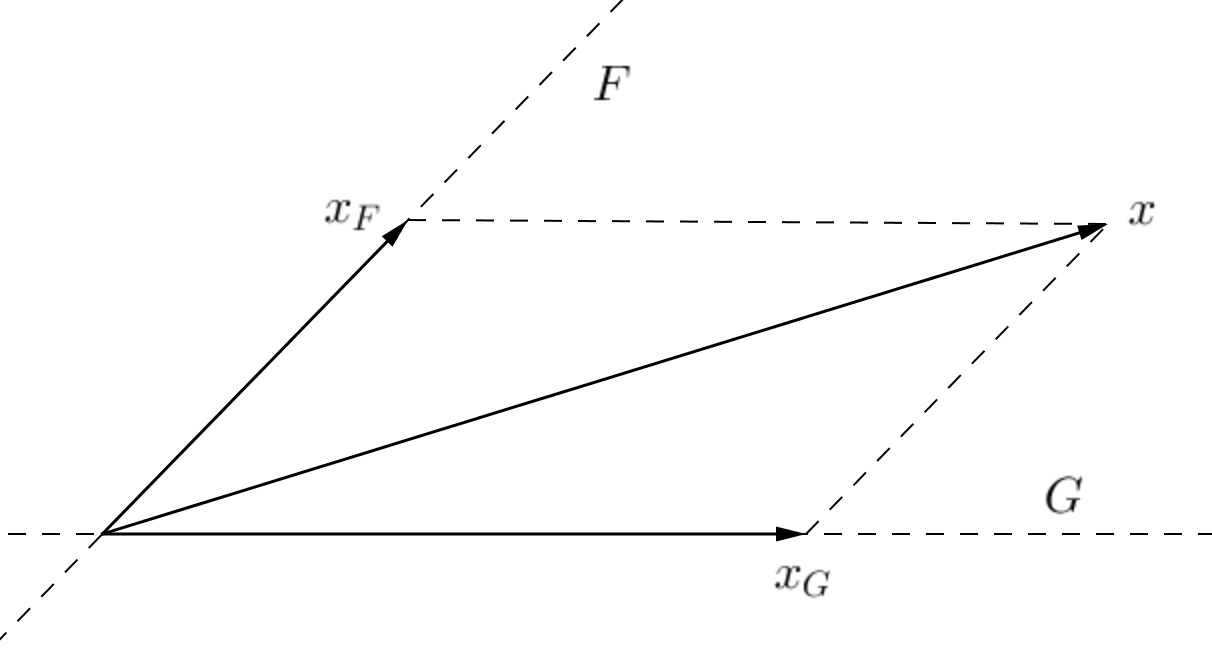
\includegraphics[scale=0.4]{Projection1}
\end{center}

\begin{nota} L'application identité de $E$ sera notée $\textrm{Id}_E$ ou plus simplement $\textrm{Id}$ si il n'y a pas d'ambiguïté.
\end{nota}

\begin{Proposition}{} Gardons les mêmes notations que dans la définition précédente. Alors :
\begin{itemize}
\item $p$ est un endomorphisme de $E$ vérifiant $p \circ p = p$.
\item $\textrm{Im}(p) = \textrm{Ker}(p-\textrm{Id})=F$ et $\textrm{Ker}(p)=G$.
\item En particulier, $E = \textrm{Im}(p) \oplus \textrm{Ker}(p)$.
\end{itemize}
\end{Proposition}

\begin{Demonstration}{}

\vspace{10cm}

\newpage
$\phantom{test}$
\vspace{14cm}

\end{Demonstration}


\begin{Remarques}{}
\begin{itemize} 
\item Pour tout $x \in E$, $x=p(x)+x-p(x)$. 
\item Si $q$ est la projection sur $G$ parallèlement à $F$ alors $p+q=\textrm{Id}$.
\end{itemize}
\end{Remarques}{}

\begin{Definition}{} On appelle \emph{projecteur} d'un espace vectoriel $E$, tout endomorphisme $p$ de $E$ vérifiant $p \circ p = p$.
\end{Definition}

\begin{Proposition}{} Soit $E$ un $\mathbb{K}$-espace vectoriel.

Un endomorphisme $p$ de $E$ est une projection si et seulement si $p$ est un projecteur. Dans ce cas, $p$ est une projection sur $\textrm{Im}(p)$ parallèlement à $\textrm{Ker}(p)$.
\end{Proposition}

\begin{Demonstration}{}
\vspace{12cm}
\newpage

$\phantom{tes}$

\vspace{11cm}
\end{Demonstration}

\begin{ApplicationDirecte} Soit $f : \mathbb{R}^3 \rightarrow \mathbb{R}^3$ définie par :
$$ f((x,y,z)=((x-z)/2,0,(z-x)/2)$$
Montrer que $f$ est un projecteur de $\mathbb{R}^3$. On précisera le noyau et l'image de $f$.
\end{ApplicationDirecte}

\begin{Definition}{} Soient $E$ un $\mathbb{K}$-espace vectoriel et $F$, $G$ deux sous-espaces vectoriels supplémentaires de $E$.

Pour tout $x \in E$, il existe un unique couple $(x_F,x_G) \in F \times G$ tel que $x=x_F+x_G$. On pose \newline $s(x)=x_F-x_G$. On définit ainsi une application $s : E \rightarrow E$ que l'on appelle \emph{symétrie vectorielle} par rapport à $F$ parallèlement à $G$. 
\end{Definition}

\begin{center}
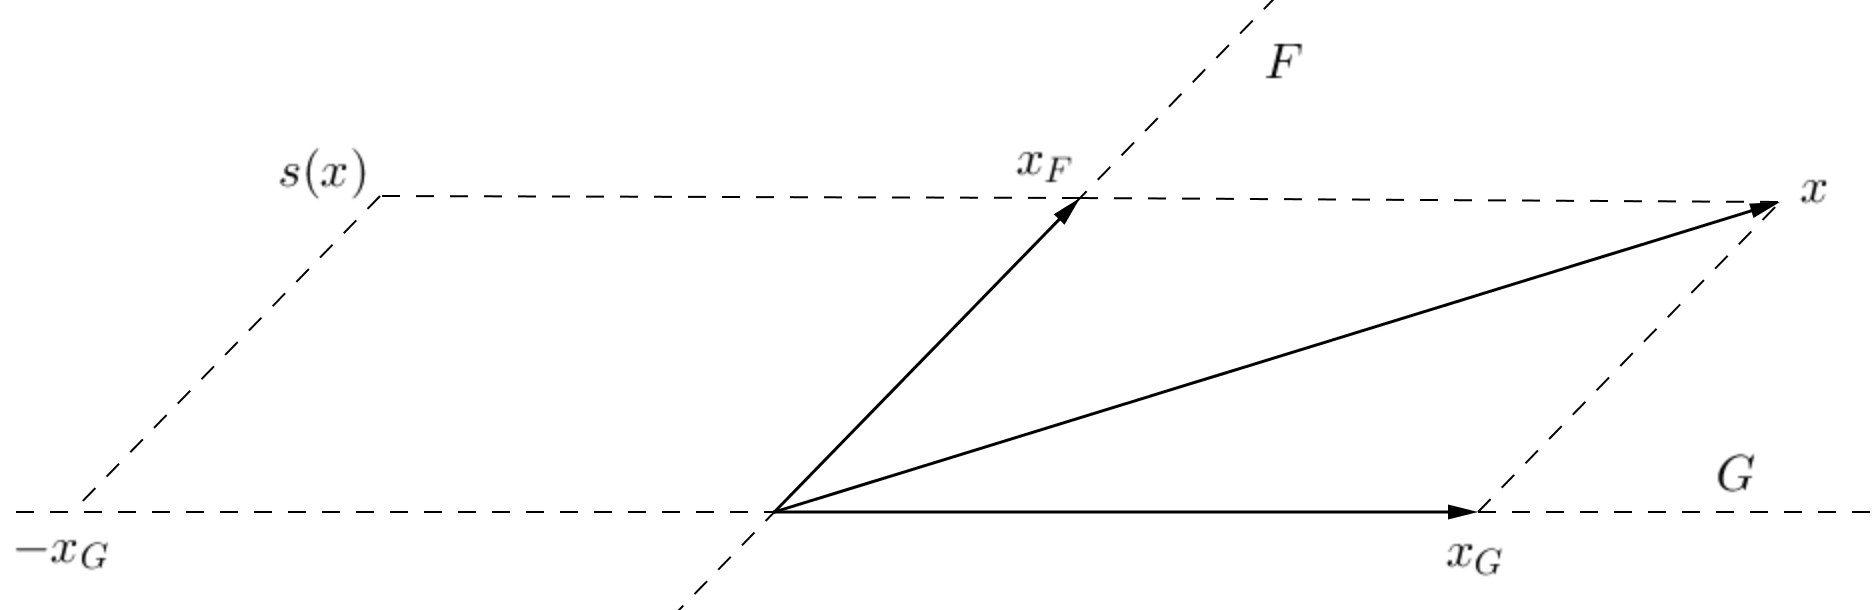
\includegraphics[scale=0.37]{Symetrie1}
\end{center}

\begin{Proposition}{} En gardant les mêmes notations que dans la définition précédente :
\begin{itemize}
\item $s$ est un endomorphisme de $E$ vérifiant $s \circ s = \textrm{Id}$.
\item $F = \textrm{Ker}(s-\textrm{Id})$ et $G= \textrm{Ker}(s+\textrm{Id})$.
\item En particulier, $E= \textrm{Ker}(s-\textrm{Id}) \oplus \textrm{Ker}(s+\textrm{Id})$.
\end{itemize}
\end{Proposition}

\begin{Demonstration}{}
\vspace{8cm}
\newpage
\phantom{test}

\vspace{7.5cm}
\end{Demonstration}

\begin{Definition}{} On appelle \emph{endomorphisme involutif} d'un espace vectoriel $E$, tout endomorphisme $s$ de $E$ vérifiant \newline $s \circ s = \textrm{Id}$.
\end{Definition}

\begin{Proposition}{} Soit $E$ un $\mathbb{K}$-espace vectoriel.

Un endomorphisme $s$ de $E$ est une symétrie si et seulement si $s$ est un endomorphisme involutif. Dans ce cas, $s$ est une symétrie par rapport à $\textrm{Ker}(p-\textrm{Id})$ parallèlement à $\textrm{Ker}(p+\textrm{Id})$.
\end{Proposition}

\vspace{13cm}

\begin{retenir} $s=2p-\textrm{Id}$
\end{retenir}


\begin{Exemple} On considère les sous-espaces vectoriels de $\mathbb{R}^3 $ suivants : $P = \left\{ {(x,y,z) \in \mathbb{R}^3 \mid x + 2y - z = 0} \right\}$ et $D = \textrm{Vect} (w){\text{ o\`u }}w = (1,0, - 1)$. Justifier l'existence de la projection vectorielle, notée $p$, sur $P$ parallèlement à $D$ puis donner son expression.

\medskip

%$\rhd$ Montrons que $P$ et $D$ sont supplémentaires pour justifier l'existence de cette projection :
%
%\begin{itemize}
%\item Soit $(x,y,z) \in \mathbb{R}^3$. On a $(x,y,z) \in P$ si et seulement si $x+2y-z=0$ ou encore $x=-2y+z$ et finalement si et seulement si $(x,y,z) = (-2y+z,y,z) = y(-2,1,0)+z(1,0,1)$. Ainsi $P = \textrm{Vect}((-2,1,0),(1,0,1))$ et $P$ est de dimension $2$ car les des vecteurs sont non colinéaires.
%\item $D$ est de dimension $1$ (car $(1,0,-1)$ est non nul).
%\item Soit $(x,y,z) \in D \cap P$. Par définition, il existe $\alpha \in \mathbb{R}$ tel que $(x,y,z)= \alpha (1,0,-1)$ et $x+2y-z=0$
%\end{itemize}

Montrons que $P$ et $D$ sont supplémentaires en raisonnant par analyse-synthèse :

%$\rhd$ \emph{Analyse} : Soit $x=(x,y,z) \in \mathbb{R}^3$. On suppose qu'il existe $(x_P,x_D) \in P \times D$ tel que $x=x_P+x_D$. Par définition de $P$, $x_p=(a,b,c)$ où $a+2b-c=0$ et par définition, il existe $\alpha \in \mathbb{R}$ tel que $x_D= \alpha (1,0,-1)$. Ainsi :
%$$ (x-\alpha, y, z + \alpha) = (a,b,c)$$
%et donc :
%$$ x- \alpha + 2y- (z + \alpha) = 0$$
%ce qui implique $\alpha = \dfrac{x+2y-z}{2}$ puis $x_D =  \dfrac{x+2y-z}{2}(1,0,-1)$ et donc $x_P = x-\dfrac{x+2y-z}{2} (1,0,-1)$.
%
%\medskip
%
%$\rhd$ \emph{Synthèse} : Soit $x =(x,y,z) \in \mathbb{R}^3$. Posons :
%$$ x_D =  \dfrac{x+2y-z}{2}(1,0,-1) \quad \hbox{ et } x_P = x-x_D$$
%On a bien $x=x_D+x_P$. Il est clair que $x_D \in D$. Vérifions que $x_P \in P$ : on a :
%$$ x_P = (x,y,z)  -\dfrac{x+2y-z}{2} (1,0,-1) = \left(x- \dfrac{x+2y-z}{2}, y, z+ \dfrac{x+2y-z}{2} \right)$$
%et :
%$$ x- \dfrac{x+2y-z}{2} + 2y - \left( z+ \dfrac{x+2y-z}{2} \right) = 0$$
%donc $x_P \in P$. Tout vecteur de $\mathbb{R}^3$ est donc somme d'un élément de $D$ et d'un élément de $P$ et cette décomposition est unique (d'après l'analyse).
%
%\medskip
%
%Ainsi $P$ et $D$ sont supplémentaires dans $\mathbb{R}^3$ donc la projection de vectorielle sur $P$ paraallèlement à $D$ existe. Le raisonnement nous fournit son expression : 
%$$ \forall (x,y,z) \in \mathbb{R}^3, \, p((x,y,z))= \left(x- \dfrac{x+2y-z}{2}, y, z+ \dfrac{x+2y-z}{2} \right) = \dfrac{1}{2} \left(x-2y+z , 2y, x+2y+z \right)$$

\vspace{22cm}
\end{Exemple}

\begin{ApplicationDirecte} Soient $F= \lbrace (x,y,z) \in \mathbb{R}^3 \, \vert \, x+y+z =0 \rbrace$ et $G= \textrm{Vect}((1,1,1))$. Justifier l'existence de la projection sur $F$ parallèlement à $G$ et donner son expression. De même avec la symétrie par rapport à $F$ parallèlement à $G$. \end{ApplicationDirecte}

\section{Hyperplans}

\begin{Theoreme}{} Soient $E$ un espace vectoriel de dimension $n$ et $H$ un sous-espace vectoriel de $E$. Les assertions suivantes sont équivalentes :

\begin{enumerate}
\item $H$ admet une droite vectorielle comme supplémentaire.
\item $H$ est le noyau d'une forme linéaire sur $E$ non nulle.
\item $\textrm{dim}(H)=n-1$.
\end{enumerate}
Quand elles sont vraies, on dit que $H$ est un \emph{hyperplan} de $E$.
\end{Theoreme}

\begin{Demonstration}{}

$\rhd$ Montrons que $1$ implique $3$. 

%Supposons que $H$ admette une droite vectorielle comme supplémentaire. Il existe donc un sous-espace vectoriel $D$ de $E$ de dimension $1$ tel que $E= H \oplus D$. On a alors :
%$$ n=\textrm{dim}(E) =  \textrm{dim}(H \oplus D) = \textrm{dim}(H) + \textrm{dim}(H) = \textrm{dim}(H)+1$$
%et donc $\textrm{dim}(H)=n-1$.

\medskip
\vspace{5cm}

$\rhd$ Montrons que $3$ implique $2$.

%Supposons que $\textrm{dim}(H)=n-1$. Considérons $(e_1, \ldots, e_{n-1})$ une base de $H$ et complétons-la en une base $\mathcal{B}$ de $E$, $(e_1, \ldots, e_{n-1},e_n)$ (Théorème de la base incomplète). Tout vecteur $x$ admet des coordonnées $(x_1, \ldots, x_{n-1},x_n)$ dans la base $\mathbb{B}$. On pose alors :
%$$ \begin{array}{ccccl}
%\varphi & : & E & \rightarrow & \mathbb{K} \\
%& & x & \mapsto & x_n
%\end{array}$$
%Il est évident que $\varphi$ est une forme linéaire. Celle-ci étant non nulle, son noyau est un sous-espace vectoriel de dimension au plus $n-1$. Or par construction, $H$ est inclus dans $\textrm{Ker}(\varphi)$ et est de dimension $n-1$. Par égalité des dimensions, on a donc $H = \textrm{Ker}(\varphi)$.

\vspace{10cm}


$\rhd$ Montrons que $2$ implique $1$.

%Supposons que $H$ soit le noyau d'une forme linéaire $\varphi$ sur $E$ non nulle. D'après le Théorème du rang, on a :
%$$ \textrm{dim}(E) = \textrm{dim}(\textrm{Ker}(\varphi)) +  \textrm{rg}(\varphi)$$
%Or $\varphi$ est non nulle donc $\textrm{rg}(\varphi) \geq 1$ et $\textrm{Im}(\varphi) \subset \mathbb{K}$ qui est de dimension $1$ donc finalement $\textrm{rg}(\varphi) =1$. On obtient alors que :
%$$ n = \textrm{dim}(H) + 1 $$
%donc $\textrm{dim}(H) = n-1$. Fixons $x_0$ un élément de $E$ n'appartenant pas à $H$. Cet élement n'est pas le vecteur nul (car il appartient à $H$) donc $D = \textrm{Vect}(x_0)$ est de dimension $1$. Ainsi la dimension de $E$ est égale à la somme des dimensions de $D$ et $H$. Montrons que $D \cap H = \lbrace 0_E \rbrace$ (ceci impliquera que $D$ et $H$ sont supplémentaires et donc le résultat souhaité). Bien entendu $\lbrace 0_E \rbrace \subset D \cap H$. Soit $x \in \mathcal{D} \cap H$. Par définition, il existe un scalaire $\alpha$ tel que $x = \alpha x_0$. On a ainsi par linéarité de $\varphi$ :
%$$ \varphi(x) = \alpha \varphi(x_0)$$
%or $x \in H = \textrm{Ker}(\varphi)$ donc $\varphi(x)=0$ et $x_0 \notin H$ donc $\varphi(x_0) \neq 0_E$ et ainsi $\alpha = 0$ et donc $x=0$. On a donc $D \cap H \subset \lbrace 0_E \rbrace$ et par double-inclusion, on a le résultat souhaité.

\vspace{12cm}

\newpage

\phantom{9cm}

\vspace{9cm}
\end{Demonstration}

\begin{Exemple} Posons $F = \left\lbrace P \in \mathbb{K}_n[X] \, \big{\vert} \, \int_{0}^1 P(x) \dx =0\right\rbrace \cdot$


\vspace{5cm}
%Alors $F$ est un hyperplan de $\mathbb{K}_n[X]$ car c'est le noyau de la forme linéaire $\varphi$ sur $\mathbb{K}_n[X]$ définie par :
%$$\varphi(P) = \int_{0}^1 P(x) \dx$$
\end{Exemple}

\begin{Proposition}{} Soient $E$ un espace vectoriel de dimension $n$ et $\varphi$, $\psi$ deux formes linéaires sur $E$. Alors $\textrm{Ker}(\varphi) = \textrm{Ker}(\psi)$ si et seulement si il existe $\lambda \in \mathbb{K}^*$ tel que $\varphi = \lambda \psi$ ($\varphi$ et $\psi$ sont \emph{proportionnelles}).
\end{Proposition}

\begin{Demonstration}{} Raisonnons par double implications.

\vspace{11cm}
%$\rhd$ Si il existe $\lambda \in \mathbb{K}^*$ tel que $\varphi = \lambda \psi$ alors pour tout $x \in E$, $\varphi(x) = 0$ si et seulement si $\psi(x)=0$ et donc $\textrm{Ker}(\varphi) = \textrm{Ker}(\psi)$.
%
%\medskip $\rhd$ Supposons que $\textrm{Ker}(\varphi) = \textrm{Ker}(\psi)$. Si $\varphi$ est nulle alors $\psi$ aussi donc $\varphi= \psi$. Supposons que $\varphi$ est non nulle et posons $H = \textrm{Ker}(\varphi) = \textrm{Ker}(\psi)$ qui est donc un hyperplan de $E$. Distinguons deux cas :
%
%\begin{itemize}
%\item Si $\textrm{dim}(E) \geq 2$. Soit $(e_1, e_2, \ldots, e_{n-1})$ une base de $H$ que l'on complète en une base $\mathcal{B}= (e_1, \ldots,e_n)$ de $E$. On a $\varphi(e_n) \neq 0$ et $\psi(e_n) \neq 0$ (sinon les applications seraient nulles). On a alors $\varphi(e_n) = \lambda \psi(e_n)$ où 
%$$ \lambda = \frac{\varphi(e_n)}{\psi(e_n)}$$
%Or pour tout $i \in \Interv{1}{n-1}$, $\varphi(e_i)=0$ et $\lambda \psi (e_i)=0$ donc $\varphi(e_i)=\lambda \psi (e_i)$. Finalement, $\varphi$ et $\lambda \psi$ coïncident sur une base de $E$ donc sont égales.
%\item Si $E$ est de dimension $1$, alors $H = \lbrace 0_E \rbrace$. Si $(e_1)$ est une base de $E$ alors $\varphi(e_1) \neq 0$ et $\psi(e_1) \neq 0$ (sinon les applications seraient nulles). On a alors $\varphi(e_1) = \lambda \psi(e_1)$ où 
%$$ \lambda = \frac{\varphi(e_1)}{\psi(e_1)}$$
%Ainsi $\varphi$ et $\lambda \psi$ coïncident sur une base de $E$ donc sont égales.
%\end{itemize}
\end{Demonstration}

\newpage

$\phantom{test}$

\vspace{3cm}

\begin{TheoremeDefinition}{} Soient $E$ un espace vectoriel de dimension finie et $H$ un hyperplan de $E$. Il existe alors une forme linéaire non nulle $\varphi$ sur $E$ telle que $H = \textrm{Ker}(\varphi)$. 

\begin{itemize}
\item On dit que l'équation $\varphi(x)=0$ est une équation de $H$. D'après la proposition précédente, l'équation de $H$ est unique à constante multiplicative non nulle près.
\item Soit $\mathcal{B}=(e_1, \ldots, e_n)$ une base de $E$. Un vecteur $x$ de coordonnées $(x_1, \ldots, x_n)$ dans la base $\mathcal{B}$ appartient à $H$ et seulement si $\varphi(x)=0$ ce qui est équivalent par linéarité de $\varphi$ à :
$$x_1 \varphi(e_1) + \cdots x_n \varphi(e_n) = 0$$
C'est ce qu'on appelle l'\emph{équation} de $H$ dans la base $\mathcal{B}$.
\end{itemize}
\end{TheoremeDefinition}

\begin{Remarque}{} En posant pour tout $i \in \Interv{1}{n}$, $a_i = \varphi(e_i)$, on a :
$$ x \in H \Longleftrightarrow a_1 x_1 + \cdots + a_n x_n = 0$$
\end{Remarque}

\begin{Exemples}
\begin{enumerate}
\item Les hyperplans de $\mathbb{R}^2$ sont de la forme :

\vspace{1cm}

%$$ \lbrace  (x,y) \in \mathbb{R}^2 \, \vert \,  ax+by = 0 \rbrace$$
où $(a,b) \neq (0,0)$. On reconnait des équations de droites vectorielles.
\item  Les hyperplans de $\mathbb{R}^3$ sont de la forme :

\vspace{1cm
}
%$$ \lbrace   (x,y,z) \in \mathbb{R}^3 \, \vert \, ax+by+cz = 0\rbrace$$
où $(a,b,c) \neq (0,0,0)$. On reconnait des équations de plans vectoriels.
\item Posons pour $n \in \mathbb{N}^*$, $H = \lbrace (x_1, \ldots, x_n) \in \mathbb{R}^n \, \vert \, x_1 + \cdots + x_n = 0 \rbrace \cdot$

Alors $H$ est un hyperplan de $\mathbb{R}^n$ car c'est le noyau de la forme linéaire non nulle suivante :
$$ \begin{array}{ccccl}
\varphi & : & \mathbb{R}^n  & \rightarrow & \mathbb{R} \\
& & (x_1, \ldots, x_n) & \mapsto &  x_1 + \cdots + x_n \\
\end{array}$$
\end{itemize}
\end{Exemples}

\begin{ApplicationDirecte} Donner rapidement la dimension de $\lbrace P \in \mathbb{R}_n[X] \, \vert P(0)+P(1)+P(2)= 0 \rbrace\cdot$ \end{ApplicationDirecte}






\end{document}
